\chapter*{Testing}
	Vediamo in questo capitolo i test eseguiti sui vari software ed algoritmi suggeriti. Diciamo innanzitutto che i test sono stati eseguiti su un sottoinsieme dei dataset proposti, in particolare abbiamo preso le prime 50k righe da ogni dataset. Abbiamo fatto questo in quanto utilizzare i dataset originali (più di 2 milioni di righe ciascuno) avrebbe richiesto tempi d'esecuzione troppo lunghi.\\
	Per i vari software e  algoritmi testati abbiamo cercato di mantenere configurazioni più simili possibile. Abbiamo specificato il massimo numero di iterazioni per ogni algoritmo (100, 200 e 400) e, negli algoritmi che supportavano parallelizzazione (ovvero il nostro Rankboost e gli algoritmi RT-Rank) sono stati parallelizzati con 50 processori.\\
	\\
	I primi test che abbiamo eseguito sono quelli relativi a 100 iterazioni massime (o massimo 100 alberi negli algoritmi tree-based).\\
	Nella Tabella \ref{tab:time_100} possiamo vedere i tempi di esecuzione totali, in secondi, dei vari algoritmi sui vari dataset.

	\begin{table}[!h]
		\centering
		\begin{tabular}{ll|r|r|r|r|r|r|}
			&& \textbf{Fold1} & \textbf{Fold2} & \textbf{Fold3} & \textbf{Fold4} & \textbf{Fold5} & \textbf{Yahoo}\\
			\hline
			\multirow{5}{*}{\textbf{Quickrank}} & \textbf{Rankboost} & $1893.44$ & $1406.33$ & $1377.14$ & $1432.61$ & $1454.83$ & $8720.14$\\
			\cline{2-8}
			& \textbf{Mart} & $27.58$ & $27.57$ & $27.34$ & $26.66$ & $28.32$ & $72.41$\\
			\cline{2-8}
			& \textbf{LambdaMart} & $28.34$ & $28.55$ & $27.99$ & $29.16$ & $28.69$ & $74.45$\\
			\cline{2-8}
			& \textbf{OBVMart} & $22.44$ & $22.49$ & $22.84$ & $22.11$ & $21.94$ & $74.90$\\
			\cline{2-8}
			& \textbf{OBVLambdaMart} & $24.42$ & $23.68$ & $23.39$ & $23.26$ & $25.24$ & $75.51$\\
			\hline
			\textbf{RankLib} & \textbf{Rankboost} & $8976.79$ & $9557.26$ & $9165.96$ & $9128.61$ & $9508.41$ & $167704.94$\\
			\hline
			\multirow{2}{*}{RT-\textbf{Rank}} & \textbf{Random Forests} & $705.14$ & $5.36$ & $4.75$ & $4.89$ & $4.95$ & $18.91$\\
			\cline{2-8}
			& \textbf{IGBRT} & $952.59$ & $28.76$ & $27.64$ & $28.31$ & $28.19$ & $51.52$\\
			\hline
			\textbf{jForests} & \textbf{LambdaMart} & $44.32$ & $42.83$ & $43.53$ & $43.35$ & $44.77$ & $146.68$\\
			\hline
		\end{tabular}
		\caption{Tempi di esecuzione (in secondi) dopo 100 iterazioni massime.}
		\label{tab:time_100}
	\end{table}
	
	Notiamo innanzitutto che gli algoritmi basati su alberi (ovvero tutti tranne Rankboost) sono estremamente più veloci. Per questo motivo abbiamo deciso di rappresentare in Figura \ref{fig:time_100_small} soltanto i tempi di esecuzione più veloci, al fine di avere una lettura più chiara.\\
	In Figura \ref{fig:time_100_percentage} vediamo invece i tempi di esecuzione in percentuale sui vari dataset per ogni algoritmo. Da questo grafico vediamo subito come il dataset Yahoo sia quello più ``impegnativo'' per i vari algoritmi, ad eccezione degli algoritmi RT-Rank che impiegano la maggior parte del tempo sul Fold1.\\
	
	\begin{figure}[!h]
		\centering
		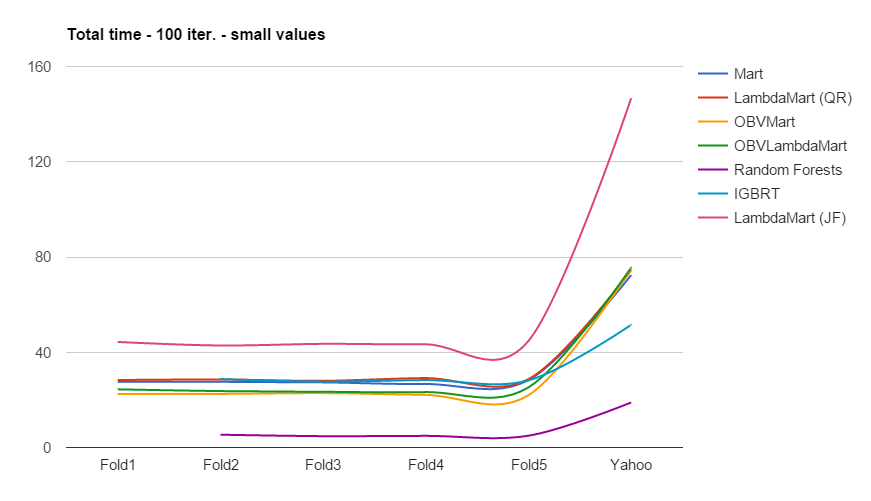
\includegraphics[scale=0.7]{time_100_small.png}
		\caption{Tempi di esecuzione bassi (in secondi) dopo 100 iterazioni massime.}
		\label{fig:time_100_small}
	\end{figure}
	
	\begin{figure}[!h]
		\centering
		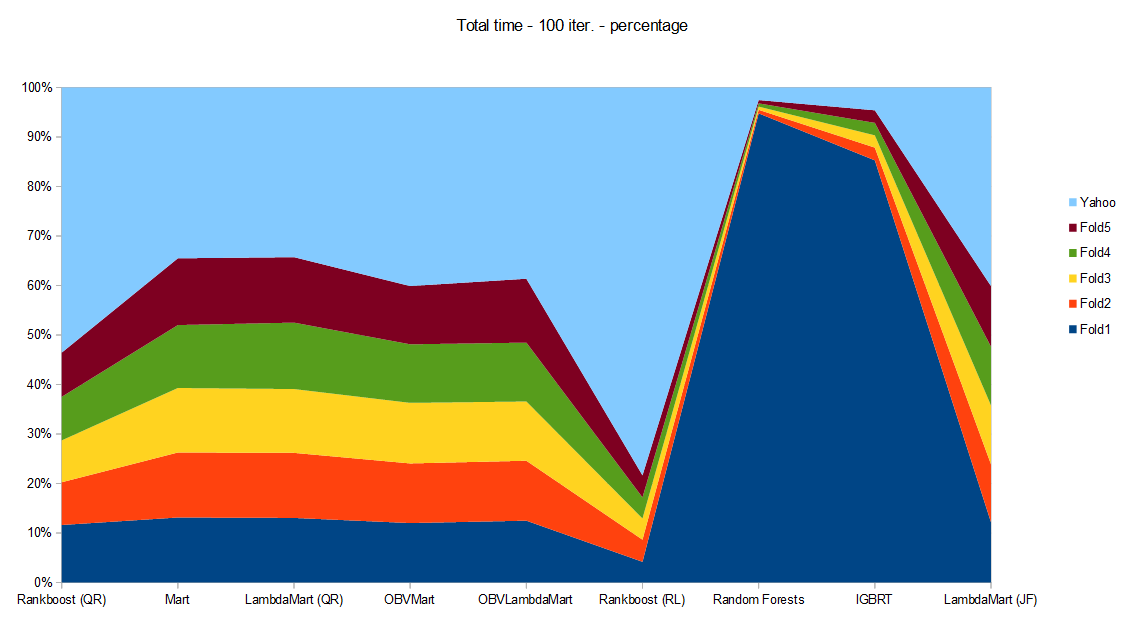
\includegraphics[scale=0.5]{time_100_percentage.png}
		\caption{Tempi di esecuzione in percentuale dopo 100 iterazioni massime.}
		\label{fig:time_100_percentage}
	\end{figure}
	
	Vediamo adesso i grafici dei valori NDCG sui set di training, validation e test per ogni algoritmo ed ogni dataset. Per chiarezza di lettura non abbiamo incluso le tabelle relative ai valori NDCG ottenuti con questi test. Per consultarli visitare il seguente indirizzo: \url{https://docs.google.com/spreadsheets/d/1vXvkFWOHsGrn0sFNtyqgyLr0Lo-dTIV9bmV4sTKwVL4/edit?usp=sharing}.\\
		
	\begin{figure}[!h]
		\centering
		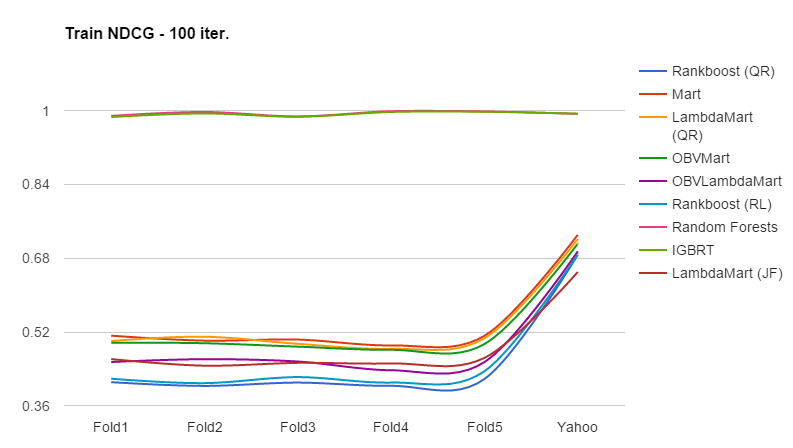
\includegraphics[scale=0.53]{train_100.png}
		\caption{Metriche NDCG del Training Set dopo 100 iterazioni massime.}
		\label{fig:train_100}
	\end{figure}
		
	\begin{figure}[!h]
		\centering
		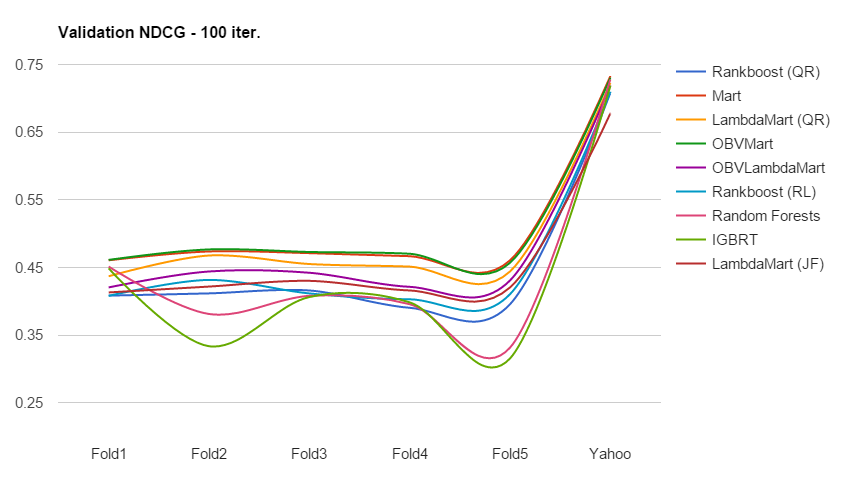
\includegraphics[scale=0.53]{validation_100.png}
		\caption{Metriche NDCG del Validation Set dopo 100 iterazioni massime.}
		\label{fig:vali_100}
	\end{figure}
			
	\begin{figure}[!h]
		\centering
		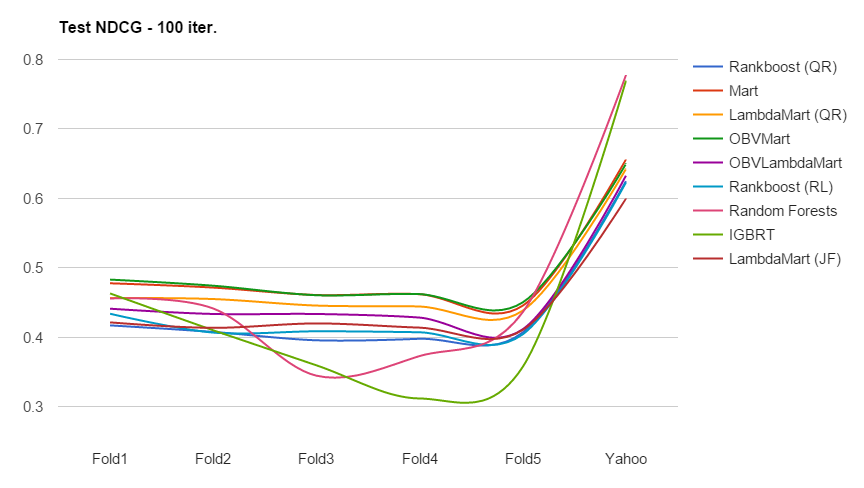
\includegraphics[scale=0.53]{test_100.png}
		\caption{Metriche NDCG del Test Set dopo 100 iterazioni massime.}
		\label{fig:test_100}
	\end{figure}
	
	Confrontando i tre grafici notiamo come gli algoritmi di RT-Rank, nonostante raggiungano valori altissimi sulla predizione del Training Set (sono le due linee in alto in Figura \ref{fig:train_100}, sovrapposte), non riescono tuttavia a raggiungere gli stessi risultati nei set di Validation e Test. Al contrario, hanno dei valori di NDCG anche più bassi rispetto agli altri algoritmi, quindi possiamo affermare che RT-Rank è il software che inferisce il peggio possibile su dati sconosciuti, imparando ``troppo'' del Training Set.\\
	Inoltre si può osservare come, in generale, la fase di boosting dell'algoritmo IGBRT peggiori i risultati già ottenuti con Random Forests, aumentando però i tempi di esecuzione.\\
	\\
	Abbiamo ripetuto i test anche con 200 e 400 iterazioni massime (per i soli algoritmi basati su alberi) ed abbiamo ottenuto risultati molto simili a questi primi test (a parte tempi d'esecuzione leggermente più lunghi). Inoltre alcuni algoritmi utilizzavano meno di 400 alberi, quindi non siamo andati oltre con i test.\\
	Non riportiamo nessuna tabella o grafico (essendo molto simili ai precedenti). Per una consultazione in dettaglio dei tempi di esecuzione e dei valori NDCG ottenuti si vada al seguente indirizzo: \url{https://docs.google.com/spreadsheets/d/1vXvkFWOHsGrn0sFNtyqgyLr0Lo-dTIV9bmV4sTKwVL4/edit?usp=sharing}.
